%%%%%%%%%%%%%%%%%%%%%%%%%%%%%%%%%%%%%%%%%%%%%%%%%%%%%%%%%%%%%%%%%%%%%%%%
% FRONTPAGE
\newpage
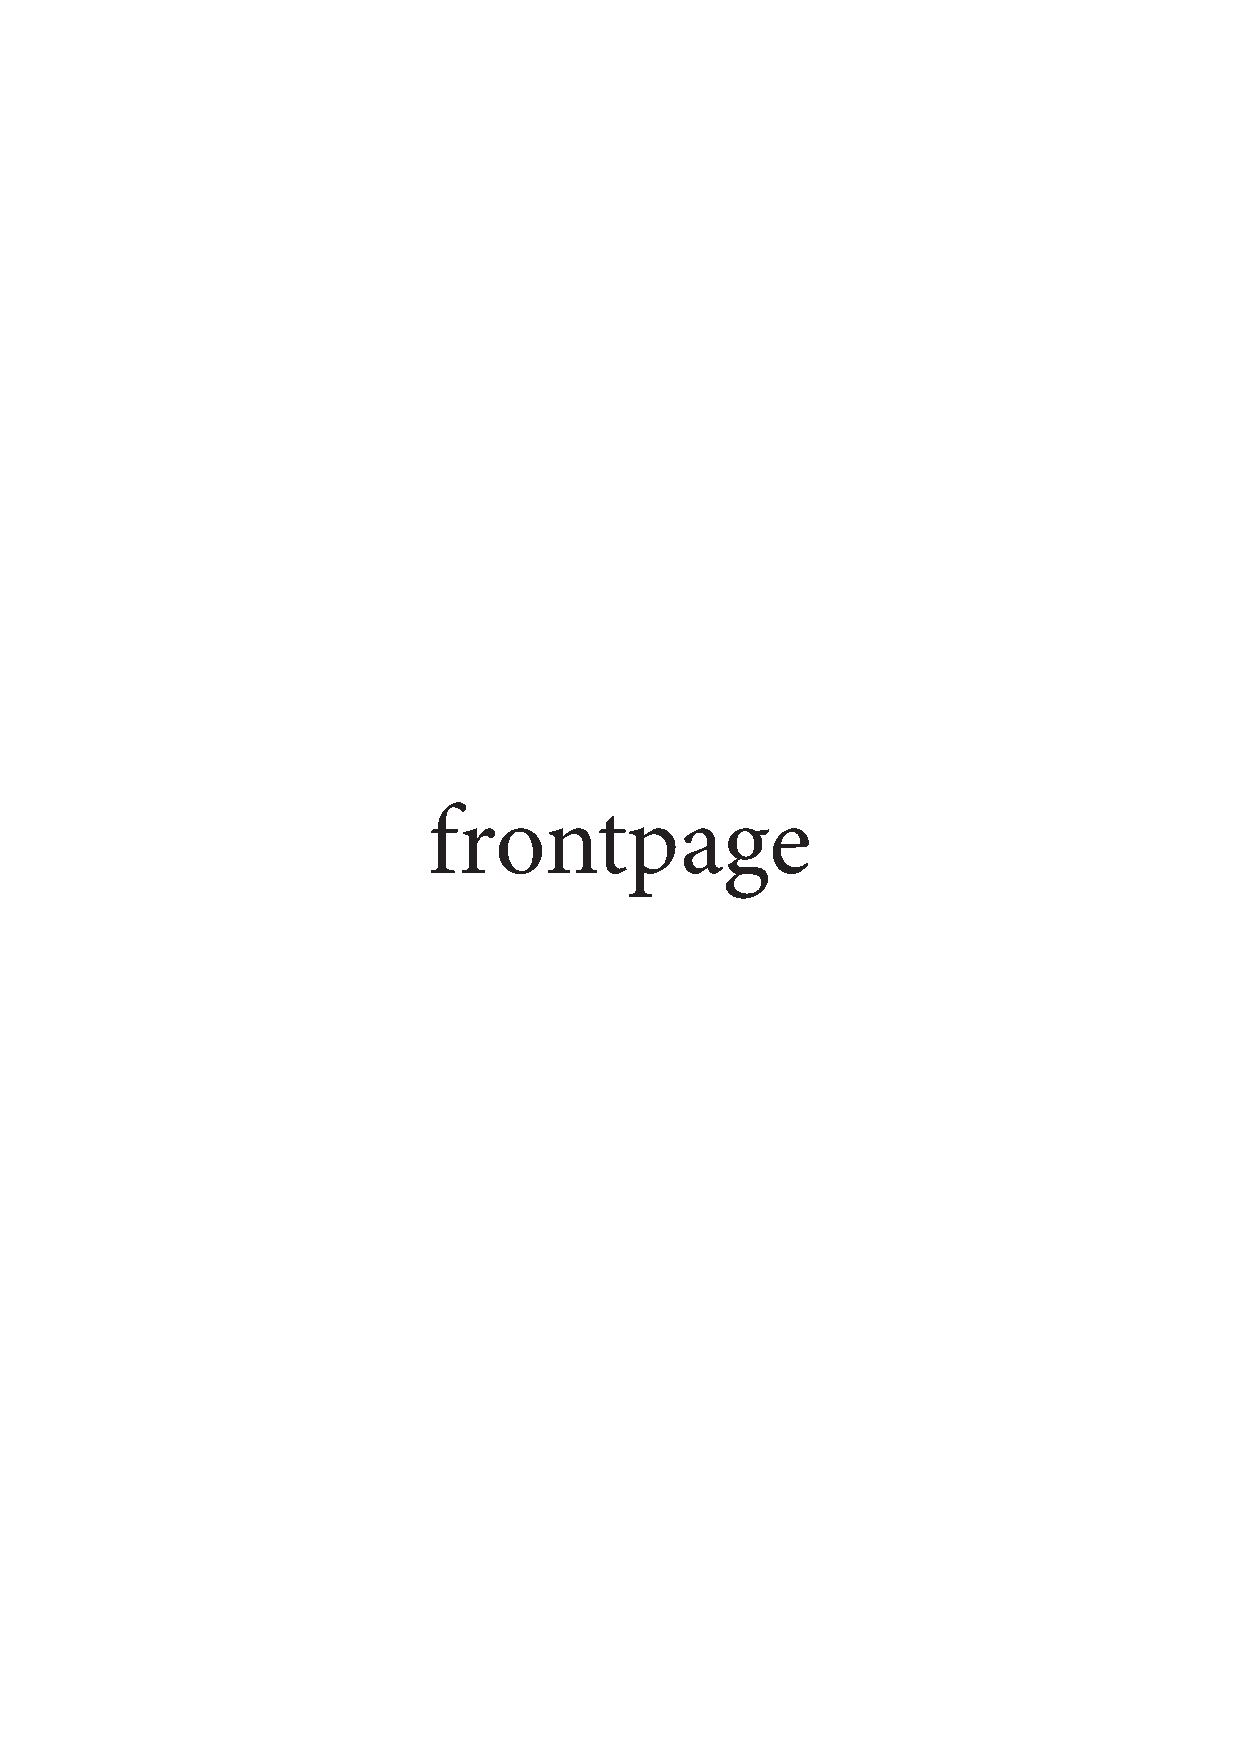
\includepdf[pages={1}]{documents/frontpage_placeholder.pdf} 
%replace your document

%%%%%%%%%%%%%%%%%%%%%%%%%%%%%%%%%%%%%%%%%%%%%%%%%%%%%%%%%%%%%%%%%%%%%%%%
% ASSIGNMENT
%\newpage
%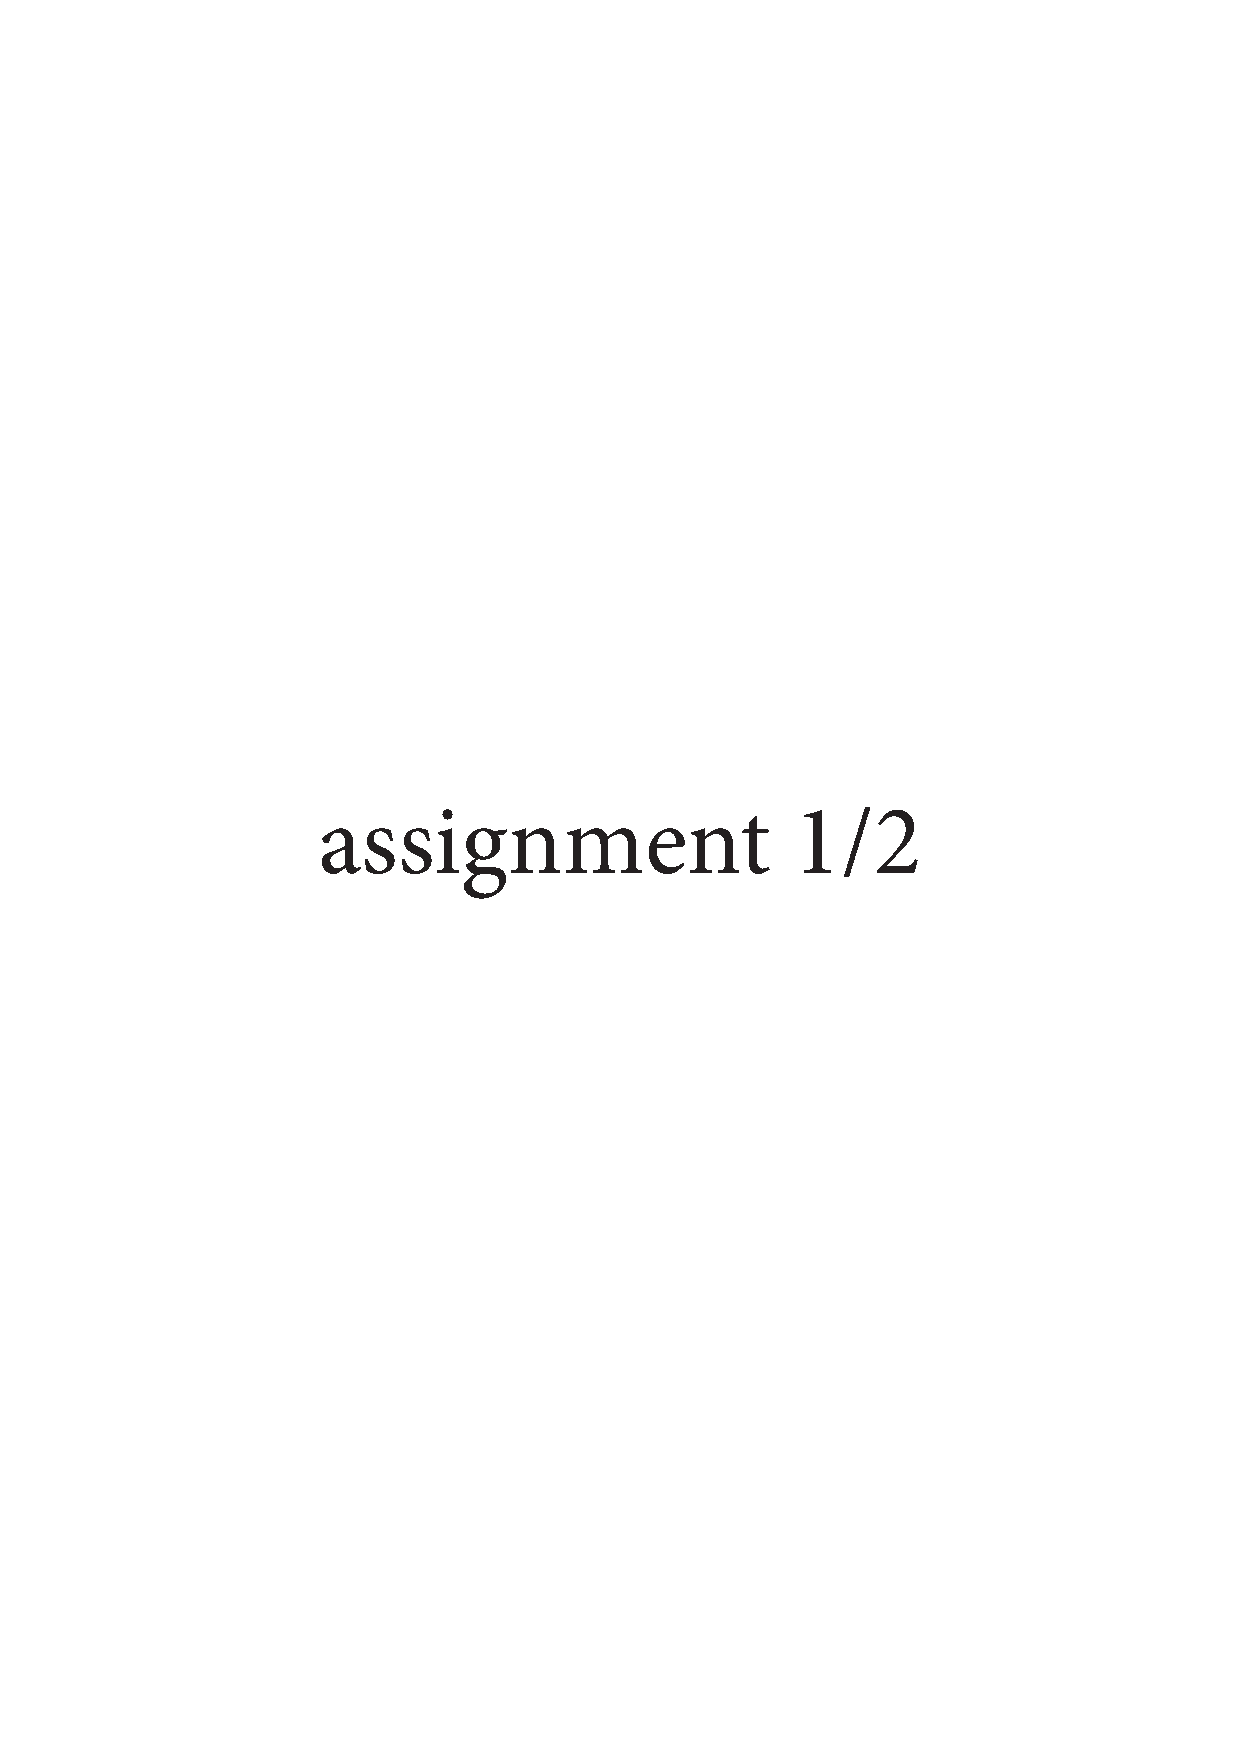
\includepdf[pages={1,2}]{documents/assignment_placeholder.pdf}
%replace your document

%%%%%%%%%%%%%%%%%%%%%%%%%%%%%%%%%%%%%%%%%%%%%%%%%%%%%%%%%%%%%%%%%%%%%%%%
% ACKNOWLEDGEMENT

\newpage
\thispagestyle{empty}

\vspace*{\fill}
\section*{ACKNOWLEDGEMENT}
\mbox
\indent I would like to very much thank my supervisor, Assoc. Ing. Ctirad Červinka, Ph.D. for his valuable advice on my way of learning the tools of computational chemistry, the opportunity to participate in real research and for the time devoted during consultations. Computational resources were provided by the e-INFRA CZ project (ID:90254), supported by the Ministry of Education, Youth and Sports of the Czech Republic.

%\vspace*{\fill}
% \noindent Práce byla podpořena projekty Grantové agentury ČR č. ...


%%%%%%%%%%%%%%%%%%%%%%%%%%%%%%%%%%%%%%%%%%%%%%%%%%%%%%%%%%%%%%%%%%%%%%%%

% SUMMARY

\newpage
\thispagestyle{empty}

\section*{SUMMARY}
Limited bioavailability of numerous active pharmaceutical ingredients is due to the poor solubility of their crystalline phases in water. The preparation of amorphous solid dispersions with biocompatible polymers offer a solution to overcome this problem, which currently limits the wider use of many drugs. This work presents a solution in the form of molecular dynamic modelling of binary systems composed of selected poorly soluble active pharmaceutical ingredients and polylactic acid as a representative of biocompatible polymer excipient. Molecular dynamics tools are used to investigate the structural and cohesive properties of pure compounds and their mixtures, with special emphasis on the analysis of molecular interactions and compatibility between drug and excipient molecules. Different simulation setups for full atomic resolution polymer simulations are validated and compared with existing experimental data, in particular glass transition temperatures and densities.

The glass transition temperature indicate the influence of atomic interactions between the drug and polymer molecules forming a more favorable amorphous binary mixture. For three of the four active pharmaceutical ingredients studied, we find that mixing them with a polylactic acid results in the formation of a more favorable amorphous binary mixture. These substances showed the highest degree of polymer-drug interactions. The development of reliable computational models evaluating drug interactions with polymeric excipients will contribute to the rational design of new drug formulations in the future.


\subsection*{keywords:}
\textit{Active pharmaceutical ingredients, Biocompatible polymer excipients, Amorphous solid dispersions, Glass transitions, Molecular dynamics}

%\bigskip %space between paragraphs
\newpage
\section*{SOUHRN}
Omezená biologická dostupnost mnoha aktivních farmaceutických látek se objevuje v důsledku špatné rozpustnosti jejich krystalických fází ve vodě. Příprava amorfních disperzí léčiv s biokompatibilními polymery nabízejí řešení k překonání tohoto problému, který v současnosti omezuje širší používání mnoha léčiv. Tato práce předkládá řešení v podobě molekulárně-dynamického modelování binárních systémů obsahujících vybrané špatně rozpustné účinné farmaceutické složky a kyselinu polymléčnou jako zástupce biokompatibilních polymerních excipientů. Nástroje molekulové dynamiky jsou použity ke zkoumání strukturních a kohezních vlastností čistých látek i jejich směsí se zvláštním důrazem na analýzu molekulárních interakcí a kompatibility mezi molekulami léčiva a pomocné látky. Ověřena jsou různá simulační nastavení pro simulace polymeru v plném atomovém rozlišení a srovnána s existujícími experimentálními daty, zejména teploty skelného přechodu a hustoty.

Na teplotě skelného přechodu se ukazuje, že míra vzájemných atomových interakcí mezi molekuly léčiva a polymeru ovlivňuje formování výhodnější amorfní binární směsi. Pro tři ze čtyř studovaných farmaceuticky aktivních látek zjišťujeme, že jejich mísením s polymléčnou kyselinou dochází k formaci výhodnější amorfní binární směsi. Tyto látky vykazovaly největší míru interakcí mezi polymerem a léčivem. Vývoj spolehlivých výpočetních modelů hodnotících interakce léčiv s polymerními excipienty přispěje v budoucnu k racionálnímu návrhu nových lékových formulací.


\subsection*{klíčová slova:}
\textit{Farmaceuticky aktivní látky, Biokompatibilní polymerní excipienty, Amorfní pevné disperze, Skelný přechod, Molekulární dynamika}


% %%%%%%%%%%%%%%%%%%%%%%%%%%%%%%%%%%%%%%%%%%%%%%%%%%%%%%%%%%%%%%%%%%%%%%%%%
% Contents
\newpage
\thispagestyle{empty}
\tableofcontents

%deleting page numbering from all of the List of Contents pages
%\addtocontents{toc}{\protect\thispagestyle{empty}}
\addtocontents{toc}{\fontsize{4mm}{4mm}\selectfont\protect\enlargethispage{\baselineskip}}
\pagenumbering{gobble}